\documentclass[a4paper]{article}

\usepackage[english]{babel}
\usepackage[utf8]{inputenc}
\usepackage{amsmath}
\usepackage{graphicx}
\usepackage[colorinlistoftodos]{todonotes}
\usepackage{float}
\usepackage{subfigure}
\usepackage{subfloat}

\title{CS294 Deep RL Assignment 3: Q Learning and Actor Critic}

\author{Mohamed Khodeir}

\date{\today}

\begin{document}
\maketitle


\section*{Part 1. Q-Learning}
\subsection*{Question 1}
\begin{figure}[H]
\centering
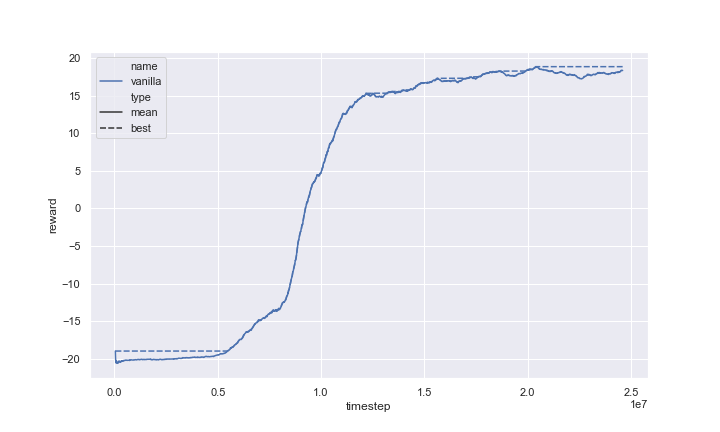
\includegraphics[width=1\textwidth]{p1q1.png}
\end{figure}


\subsection*{Question 2}
\begin{figure}[H]
\centering
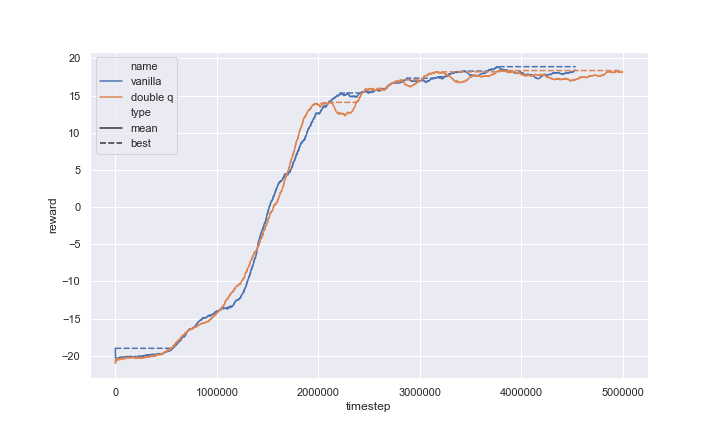
\includegraphics[width=1\textwidth]{p1q2.png}
\end{figure}

\subsection*{Question 3}
\begin{figure}[H]
\centering
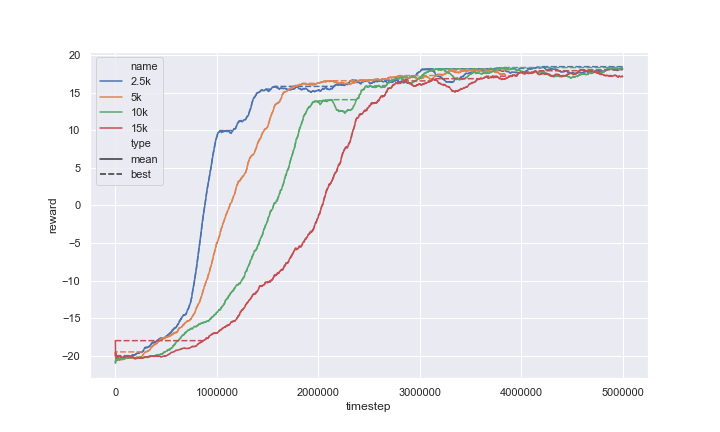
\includegraphics[width=1\textwidth]{p1q3.png}
\end{figure}


\section*{Part 2. Actor Critic}
\subsection*{Question 1}
\begin{figure}[H]
\centering
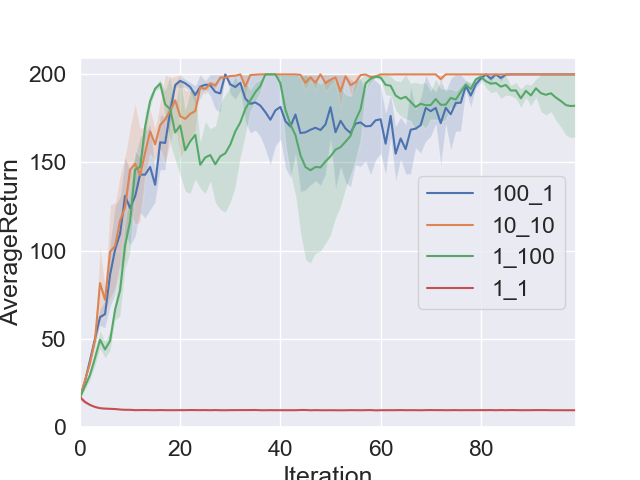
\includegraphics[width=1\textwidth]{p2q1.png}
\end{figure}


\subsection*{Question 2}
\begin{figure}[H]
\centering
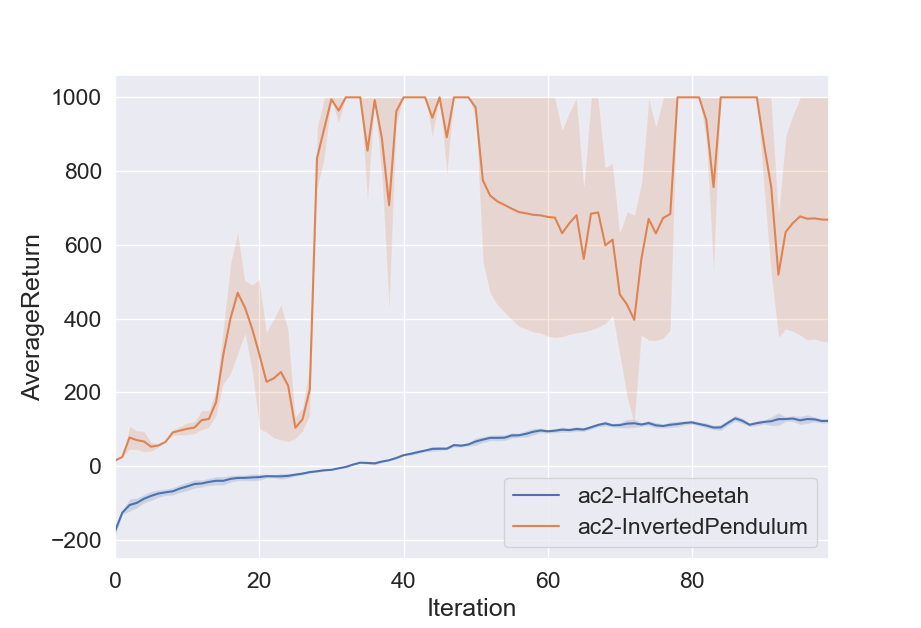
\includegraphics[width=1\textwidth]{p2q2.png}
\end{figure}

\subsection*{Bonus}
\begin{figure}[H]
\centering
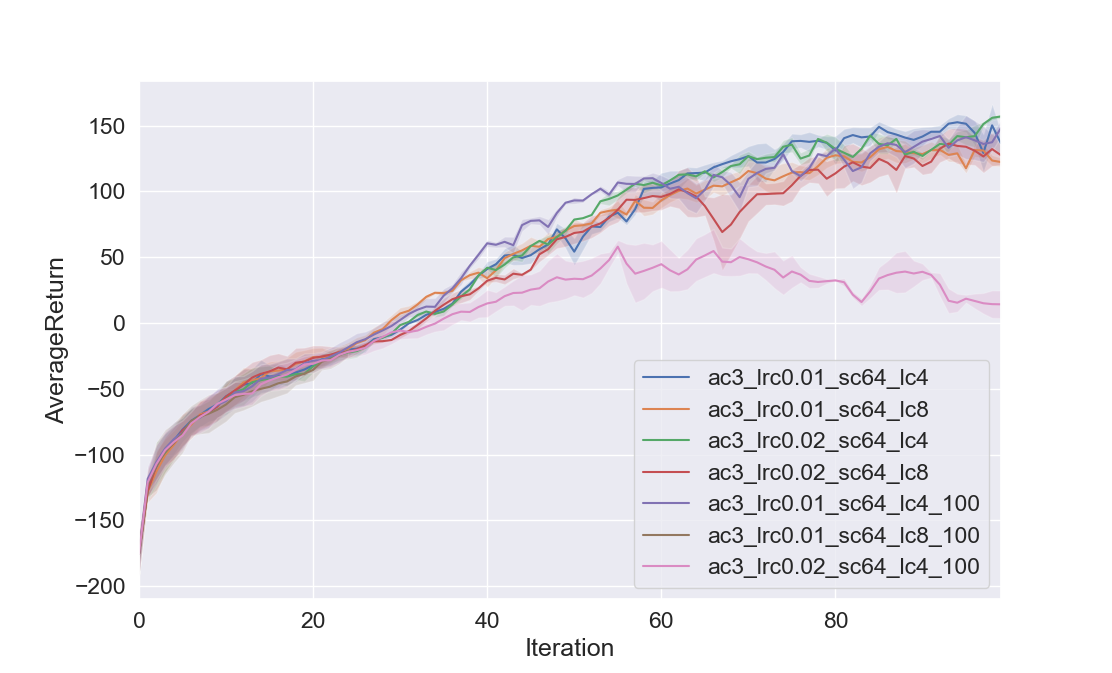
\includegraphics[width=1\textwidth]{p2q3.png}
\end{figure}
\end{document}
